\documentclass[10pt]{article}
\usepackage[margin=16mm]{geometry}
\usepackage{pgfplots}
\pgfplotsset{compat=1.18}
\pagestyle{empty}
\begin{document}
\begin{center}
{\large Rolling: discovered states for individual replacement}\par\medskip
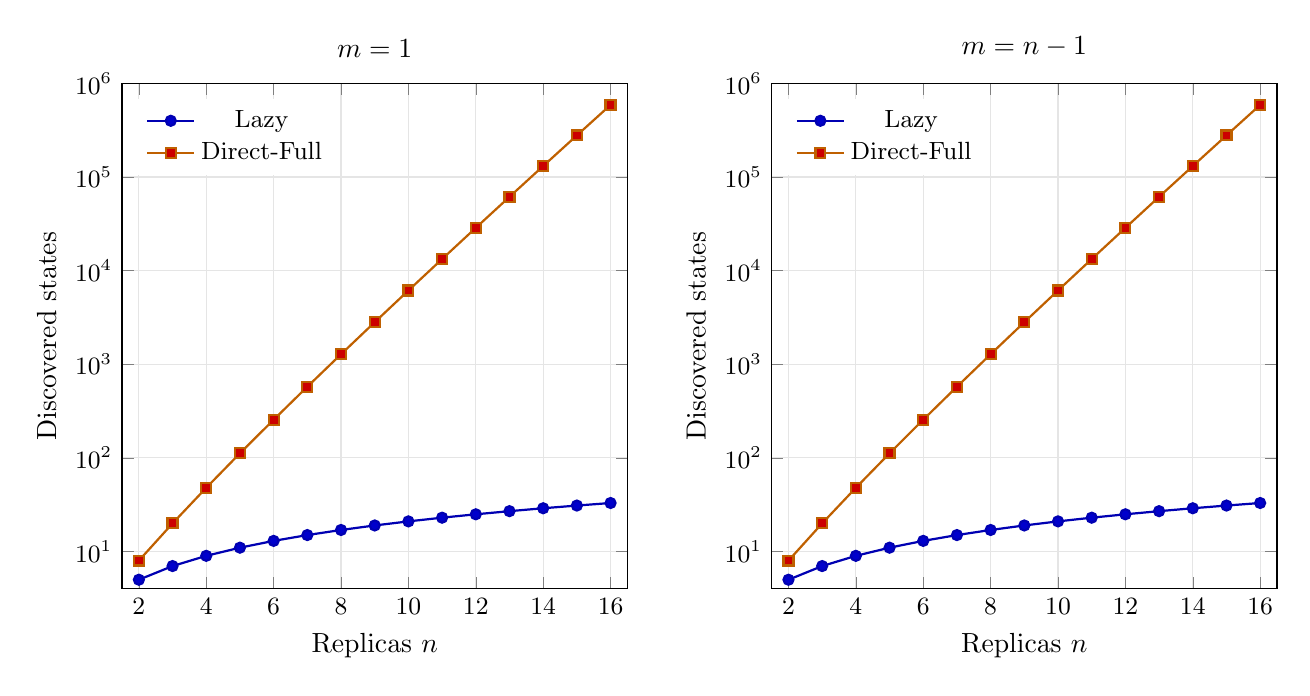
\begin{tikzpicture}
\begin{axis}[at={(0cm,0)},anchor=south west,width=8cm,height=8cm,title={$m=1$},xlabel={Replicas $n$},ylabel={Discovered states},ymode=log,log basis y=10,xmin=1.5,xmax=16.5,ymin=4,ymax=1000000,xtick={2,4,6,8,10,12,14,16},ytick={10,100,1000,10000,100000,1000000},grid=major,grid style={gray!20},legend pos=north west,legend style={font=\small,draw=none},tick label style={font=\small}]
\addplot+[thick,blue!70!black,mark=*,mark size=1.8pt] coordinates {(2,5) (3,7) (4,9) (5,11) (6,13) (7,15) (8,17) (9,19) (10,21) (11,23) (12,25) (13,27) (14,29) (15,31) (16,33)};
\addlegendentry{Lazy}
\addplot+[thick,orange!75!black,mark=square*,mark size=1.8pt] coordinates {(2,8) (3,20) (4,48) (5,112) (6,256) (7,576) (8,1280) (9,2816) (10,6144) (11,13312) (12,28672) (13,61440) (14,131072) (15,278528) (16,589824)};
\addlegendentry{Direct-Full}
\end{axis}
\begin{axis}[at={(8.25cm,0)},anchor=south west,width=8cm,height=8cm,title={$m=n-1$},xlabel={Replicas $n$},ylabel={Discovered states},ymode=log,log basis y=10,xmin=1.5,xmax=16.5,ymin=4,ymax=1000000,xtick={2,4,6,8,10,12,14,16},ytick={10,100,1000,10000,100000,1000000},grid=major,grid style={gray!20},legend pos=north west,legend style={font=\small,draw=none},tick label style={font=\small}]
\addplot+[thick,blue!70!black,mark=*,mark size=1.8pt] coordinates {(2,5) (3,7) (4,9) (5,11) (6,13) (7,15) (8,17) (9,19) (10,21) (11,23) (12,25) (13,27) (14,29) (15,31) (16,33)};
\addlegendentry{Lazy}
\addplot+[thick,orange!75!black,mark=square*,mark size=1.8pt] coordinates {(2,8) (3,20) (4,48) (5,112) (6,256) (7,576) (8,1280) (9,2816) (10,6144) (11,13312) (12,28672) (13,61440) (14,131072) (15,278528) (16,589824)};
\addlegendentry{Direct-Full}
\end{axis}
\end{tikzpicture}
\end{center}
\noindent All plotted points are completed single-trial measurements with the same fixed E1 solver JAR. Both availability extremes are shown; no analytical values fill a missing point. The vertical axes are logarithmic. Rank and adverse outcomes remain in the complete CSV tables.
\par\medskip\noindent Each component has one old and two new local states. The interval tester has $n-m+2$ states and $2n(n-m+1)$ explicitly listed changes, so the input representation is polynomial in $n$. The full-game state-count formula $(n+2)2^{n-1}$ is checked separately against observations, and is not substituted for them.
\end{document}
